%!TEX root = ../Thesis.tex
\chapter{Background}\label{cha:background}
%
\textcolor{red}{Research projects should always be based on previous research on the same and/or related topics. This should be described as a background to the thesis with adequate bibliographical references. If the material needed is too voluminous to fit nicely in the review part of the introduction, it can be presented in a separate background chapter.}


\section{Motivation}\label{sec:motivation}

The last decades traditional television viewing numbers have steadily been declining \cite{ssb_seertall}. People do not find TV as appealing as they once did. Today, more people seem to find more engaging and personal forms of entertainment elsewhere. Currently, the only form of doing, what one could call an engaging TV broadcast, is through the use of social media and hybrid broadcast broadband TV by incorporating comments, videos and audio from the audience into the TV broadcast. Sadly, this form of engagement is quite limited and does not give proficient results. 

\section{AdMiRe}\label{sec:admire}
Wanting to innovate and create better experiences in this space, the AdMiRe \cite{admire} (Advanced Mixed Realities) project has been formed as a collaboration between Brainstorm, Disguise, NTNU, EPFL, UPF, NRK, Premiere, TVR and CSIC. The aim of the AdMiRe project is to use mixed reality solutions to enable audiences at home to be incorporated into live TV programs and interact with the other people in the TV studio. 

Doing this using the available technology is hard because of the technical challenges. To make this easier AdMiRe is set out to develop and simplify key modules. 

\begin{figure}[H]
  \centering
  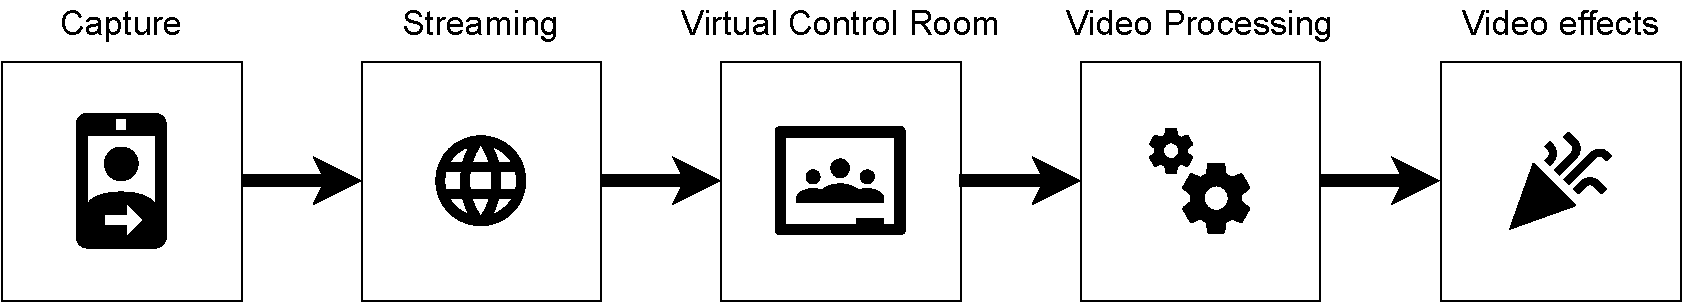
\includegraphics[width=0.9\textwidth]{img/admire_system.pdf}
  \caption{AdMiRe system flow}
  \label{fig:admire_system}
\end{figure}


An important aspect of this technology is to make it look like the participant is in the studio, and to make it look like the participant is in the studio, the participant has to be extracted out of its own environment and inserted naturally into the studio environment. That's why we will take a look at the machine learning silhouette extraction module currently used in the AdMiRe project. We will try to evaluate the quality of experience and generally assess the quality of the technology by running some objective and subjective tests on the silhouette extraction. 


\subsection{\acrlong{mlbfe}}\label{sec:mlbfe}
The AdMiRe project is using a \acrlong{mlbfe} algorithm which has been developed by the multimedia signal processing group of EPFL. 

The algorithm is MobileNet-UNet constellation. This constellation is constructed of a U-Net based autoencoder, where the encoder part has been replaced with a MobileNetV2 architecture. 

\subsubsection{U-Net}\label{sec:unet}
A U-Net architecture is a pipeline of compressions, using pooling layers, and decompressions, using transposed convolution layers \cite{ronneberger2015unet}. \autoref{fig:unet} gives a simplified 3-level illustration of this architecture. The pooling layers are used to reduce the dimensionality of the input, while the transposed convolution layers will increase the dimensionality. Each layer also gives a skip connection to the matching output layer for information retention. Information from each level contributes to the final reconstruction where convolution layers merge the final information. One of the highlights of this architecture is the low loss function.  

\begin{figure}[H]
  \centering
  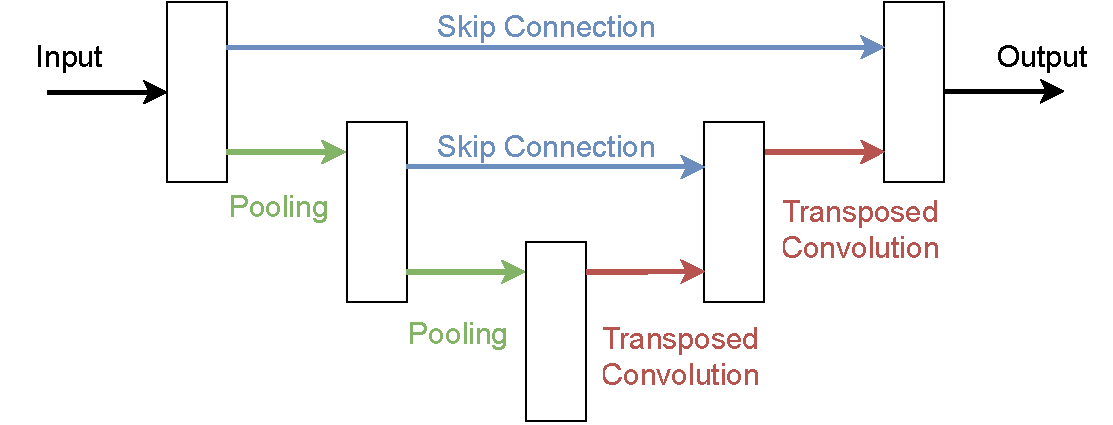
\includegraphics[width=0.9\textwidth]{img/ML/unet.pdf}
  \caption{Simplified U-Net architecture. }
  \label{fig:unet}
\end{figure}

\subsubsection{MobileNetV2}\label{sec:mobilnet}
MobileNetV2 is an improvement \cite{sandler2019mobilenetv2} of the original MobileNet \cite{howard2017mobilenets}. MobileNet is a lightweight architecture satiable for low computational power use cases using depth-wise separable convolution. 

MobileNetV2 was introduced to improve the performance. It did this by including some changes to the structure of the convolution layers with the introduced a point wise convolution layer with a linearity to the beginning of the layers \cite{vision_based}. Each layer also has a ReLU and a residual bottleneck connection is used to reduce the input size. ReLUs, Rectified Linear Units, is an  activation function which is zero in the negative dimension, but linear in the positive. A simplified illustration of the architecture of the MobileNetV2 model can be found in \autoref{fig:mobnetv2}.

\begin{figure}[H]
  \centering
  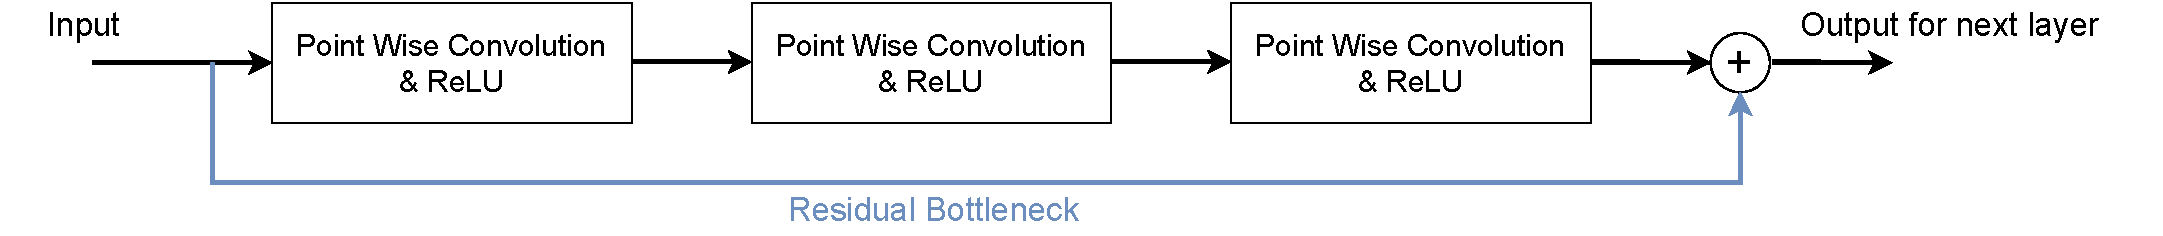
\includegraphics[width=1\textwidth]{img/ML/MobileNetV2.pdf}
  \caption{Simplified MobileNetV2 architecture. }
  \label{fig:mobnetv2}
\end{figure}

\subsubsection{MobileNet-UNet}\label{sec:mobilenet-unet}
With the combination of the two methods discussed in \autoref{sec:unet} and \autoref{sec:mobilnet}, one gets a architecture which decodes up-sampled features using transposed convolution layers with corresponding down-sampling stages \cite{8575250}. Each layer gets fused with it's corresponding layer with an element-wise addition. A simplified version of the architecture is illustrated in \autoref{fig:mobilenet-unet}. 

\begin{figure}[H]
  \centering
  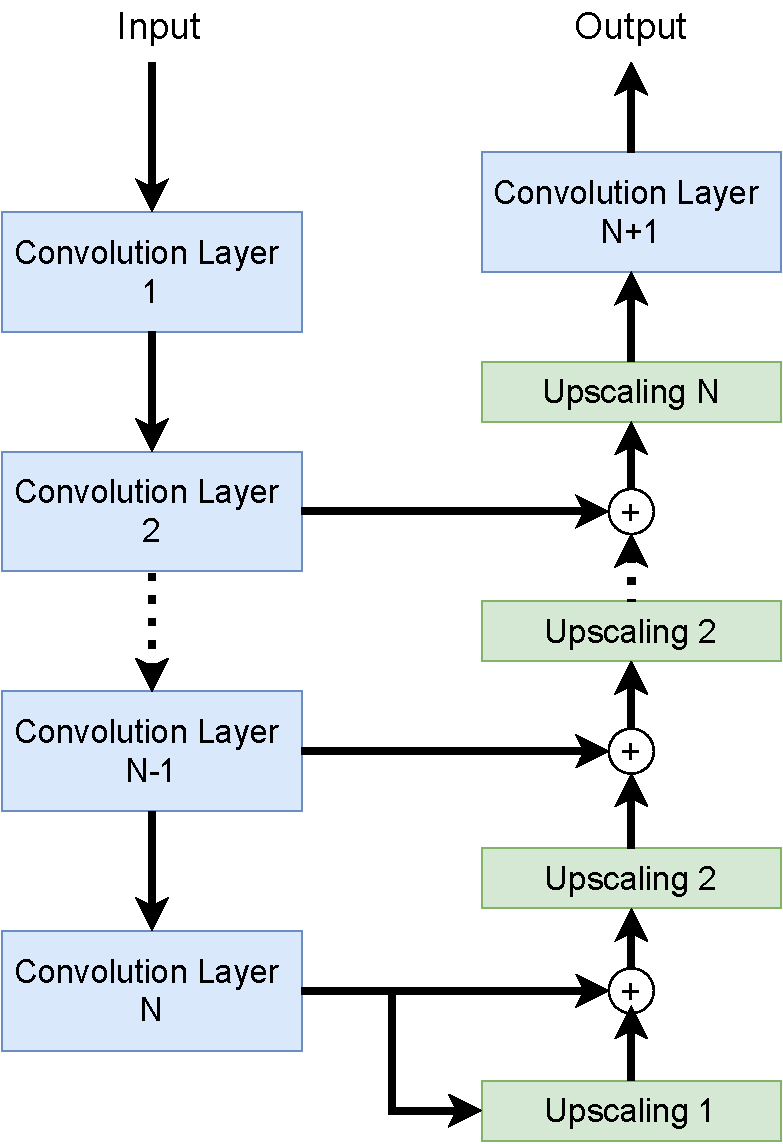
\includegraphics[width=.4\textwidth]{img/ML/MobileNet-UNet.pdf}
  \caption{Simplified MobileNet-UNet architecture. }
  \label{fig:mobilenet-unet}
\end{figure}

\subsubsection{Training, validation and testing}
The learning architecture of the model is based on the model used in \cite{bmshj2018}, with a optimisation for \acrfull{ssim}. \acrshort{ssim} is a method for predicting the perceived quality of digital signals where degradation is viewed as perceived change in structural information. The Multi Scale version is conducted over multiple samples, with multiple stages of sub-sampling \cite{mssssim}. The architecture is further using the pre-trained models available from TenserFlows Compression \cite{tensorflow_compression}.

The model has been trained, validated and tested with the human segmentation data set presented in \cite{gmnu21}. In this data set, humans have been set as foreground, while the rest of the frame is set as the background. Using this data set, the model has been trained on semantic segmentation of humans with object removal, in this case being the entire background


\section{Previous work}

\subsection{Quality of Experience}
\label{sec:qoe}
QUALINET white papers defines Quality of Experience as following \cite{book_QoE}

\begin{quote}
The degree of delight or annoyance of the user of an application or service. It results from the fulfilment of his or her expectations with respect to the utility and/or enjoyment of the application or service in the light of the user’s personality and current state.
\end{quote}

Quality of Experience is a field which is based on multiple disciplines such as social psychology, cognitive science, economics and engineering service with a focus on understanding overall human quality requirements.

There are a number of influencing factors in regards of the general Quality of Experience, namely human, system and contextual influencing factors \cite{factors_QoE}.
\begin{itemize}
    \item \textbf{Human influencing factors} (HIF) can be divided into two parts — low level and high level. Low level factors are factors such as age, physical form, emotions and mental constitution, while high level are factors such as previous knowledge regarding the matter. 
    \item \textbf{System influencing factors} (SIF) which is the technical elements in role. The type of content being consumed, what kind of media (meaning factors such as encoding, resolution, sample rate), network constrains (e.g. bandwidth, delay and jitter) and device differences (e.g. different screen sizes, resolutions, frame rate and audio quality)
    \item \textbf{Context influencing factors} (CIF) are the surrounding factors which affects the user. The physical location (e.g. lighting and surrounding space), social relationships (e.g. inter-personal relationships), type of task, interruptions, time of day, how many times the user has been using these type of systems before and more technical contextual challenges (e.g. a system which has to work together with other separate systems) are all influencing aspects.
\end{itemize}
\todo{Part from project thesis. What do we do about it? Rewrite? Declare its origin?}

\subsection{Semantic Segmentation}
When doing semantic segmentation, we mean assigning each pixels in an image a semantic class label \cite{csurka2013good}. Semantic segmentation has several use cases, such as scene understanding, object removal and local class based image enhancement. The different use cases require different level of segmentation, because of their complexity. Scene understanding might need a rougher segmentation, than what object removal might need. This makes semantic segmentation difficult to evaluate. What makes a good segmentation is entirely up to the use case and the success of the segmentation is measured by the success of the end application \cite{csurka2013good}.


\subsection{Subjective Measurement}
\label{sec:measurement}
In a use case where we want to extract the silhouette of a human to be inserted into another setting, the overall quality of the video can be strongly subjective. Since a silhouette extraction can be prone to seemingly random cuts and jitter, the perceived quality of the video from a human perspective can be strongly compromised even though objective quality measures gives a strong measure. 

\subsubsection{Mean Opinion Score and Likert Scale}
\label{sec:mos}
The Mean Opinion Score (MOS) \cite{Streijl2016} and Likert scale \cite{likert_scale} is widely used measurement for media signals and quality. This  measure is often represented as a 5-point answer system, represented in \autoref{tab:rating_label}. While these are popular methods, the usefulness is often debated due to inherent limitations of measurements in a single scalar value \cite{wiki_mos}. 

The subjective quality evaluation requires a lot of human resources and can be time consuming. The mean opinion score method is otherwise prone to misuse or misinterpretation, as the design of the subjective experiments have an important influence. The objective media quality metrics do also rely on data from the subjective experiments for tuning and validation, and it can therefore be challenging to make meaningful measurements and interpret the resulting findings correctly \cite{Streijl2016}.


\begin{table}[]
    \centering
    \begin{tabular}{ |c|c|c|c|c|c| } 
         \hline
         \textbf{Rating} & 1 & 2 & 3 & 4 & 5 \\
         \hline
         \textbf{Label} & Bad & Poor & Fair & Good & Excellent \\ 
         \hline
    \end{tabular}
    \caption{Rating and labels for subjective answers}
    \label{tab:rating_label}
\end{table}

\subsection{Objective measurement}\label{sec:objective_measurement}
Objective measurements are pixel wise comparisons of the pixels in the resulting images, up against a given truth table. The coming sections present some of the most popular measures. 

\subsubsection{\acrlong{pa}}
\acrfull{pa} is a simple measure which takes the number of correctly classified pixels, the number of \acrlong{tp} and \acrlong{tn}, over the total number of pixels in an image, the number of \acrlong{tp}, \acrlong{tn}, \acrshort{fp} and \acrshort{fn}. Easily said its the percentage of correctly classified pixels in an image \cite{jeremy}.

\begin{equation}
    \acrlong{pa} = \frac{\acrshort{tp}+\acrshort{tn}}{\acrshort{tp}+\acrshort{tn}+\acrshort{fp}+\acrshort{fn}}
\end{equation}

While this is a simple and effective measurement, it is prone to class imbalance \cite{tiu}. This can lead to a high score even though the classification itself is bad. \autoref{fig:pa} highlights this problem. The ground truth to the left has a white section in the middle, but the classifier has been unable to classify this area correctly. Since the white area in the ground truth only covers 1\% of the image, we get a 99\% pixel accuracy even though the classifier has completely failed to classify the segment.

\begin{figure}[H]
  \centering
  
\includegraphics[width=0.9\textwidth]{img/objective_measures/pa.pdf}
  \caption{Truth table to the left, and classified results to the right}
  \label{fig:pa}
\end{figure}

\subsubsection{\acrlong{iou}}
\acrfull{iou}, also known as the Jaccard index originally developed by Paul Jaccard \cite{jaccard}, has become the standard performance measure of image semantic segmentation\cite{Rezatofighi_2019_CVPR}. The measure outputs a percentage of overlap between the predicted region and the ground truth of a image segmentation. This is a count based measure looking at the intersection of the predicted and the ground truth over the union of the predicted area and ground truth. If we have a binary classification problem, we can use the number of \acrlong{tp} over the number of \acrlong{fp}, \acrlong{fn} and \acrlong{tp}.
\cite{10.1007/978-3-319-50835-1_22}

\begin{equation}
    IoU = \frac{intersection}{union} = \frac{|target \cap prediction|}{|target \cup prediction|} = \frac{\acrshort{tp}}{\acrshort{fp} + \acrshort{fn} + \acrshort{tp}}
\end{equation}


\begin{figure}[H]
  \centering
  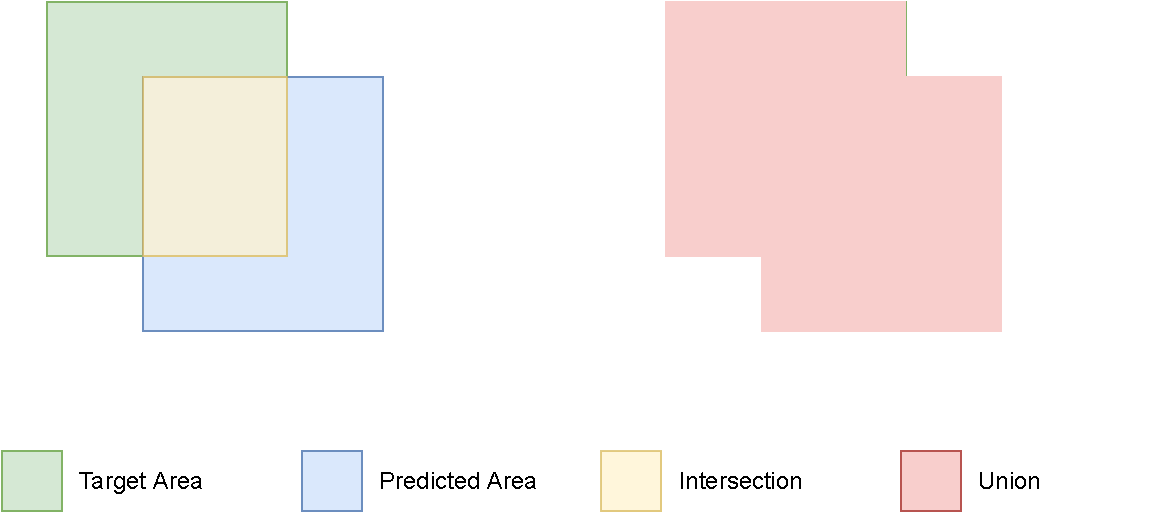
\includegraphics[width=0.9\textwidth]{img/objective_measures/iou.pdf}
  \caption{Intersection over Union}
  \label{fig:iou}
\end{figure}

\subsubsection{\acrlong{dc}}
The \acrfull{dc} is a similar metric to \acrlong{iou}. Like \acrlong{iou}, \acrlong{dc} is a statistic used to measure the similarity between two samples \cite{sorensen}\cite{dice}. The measure outputs a percentage between two times the overlap and the total number of pixels in both images, as seen in \autoref{eq:dc} and illustrated in \autoref{fig:dc}. For a binary classification the measure outputs a percentage of two times the number of \acrlong{tp} and the total of two times the \acrlong{tp}, \acrlong{fp} and \acrlong{fn}.

\begin{equation}\label{eq:dc}
    \acrshort{dc} =  \frac{2|target \cap prediction|}{|target| + |prediction|} = \frac{2\acrshort{tp}}{2\acrshort{tp}+ \acrshort{fp} + \acrshort{fn}}
\end{equation}

\acrlong{dc} and \acrlong{iou} will always be positively correlated for a fixed ground truth, and will always be within a factor of two of each other, as stated in \autoref{eq:dc_iou_relation}.

\begin{equation}\label{eq:dc_iou_relation}
    \frac{\acrshort{dc}}{2} \leq \acrshort{iou} \leq \acrshort{dc}
\end{equation}

While \acrlong{iou} tends to penalise single instances of bad classification more than the \acrlong{dc}. The \acrlong{dc} works better for measuring the average performance of a parameter. For example, imagine we have two classifiers, A and B. If A were to be a great classifier, but had one bad classification, the average \acrlong{iou} score, would be penalised much harder than the average \acrlong{dc}, since this is not so prone to outlier values. This would result in giving the impression that B might be a better classifier than A, if we were only to look at the \acrlong{iou} \cite{276144}.

\acrlong{dc} \textbf{(S)} being so similar to \acrlong{iou} \textbf{(J)} and can easily be converted using the relations in \autoref{eq:iou-dc} and \autoref{eq:dc-iou} \cite{wiki_dc}.

\begin{minipage}{.45\linewidth}
\begin{equation}\label{eq:iou-dc}
    J = \frac{S}{2 - S}
\end{equation}
\end{minipage}
\begin{minipage}{.45\linewidth}
\begin{equation}\label{eq:dc-iou}
    S = \frac{2J}{1 + J}
\end{equation}
\end{minipage}

\begin{figure}[H]
  \centering
  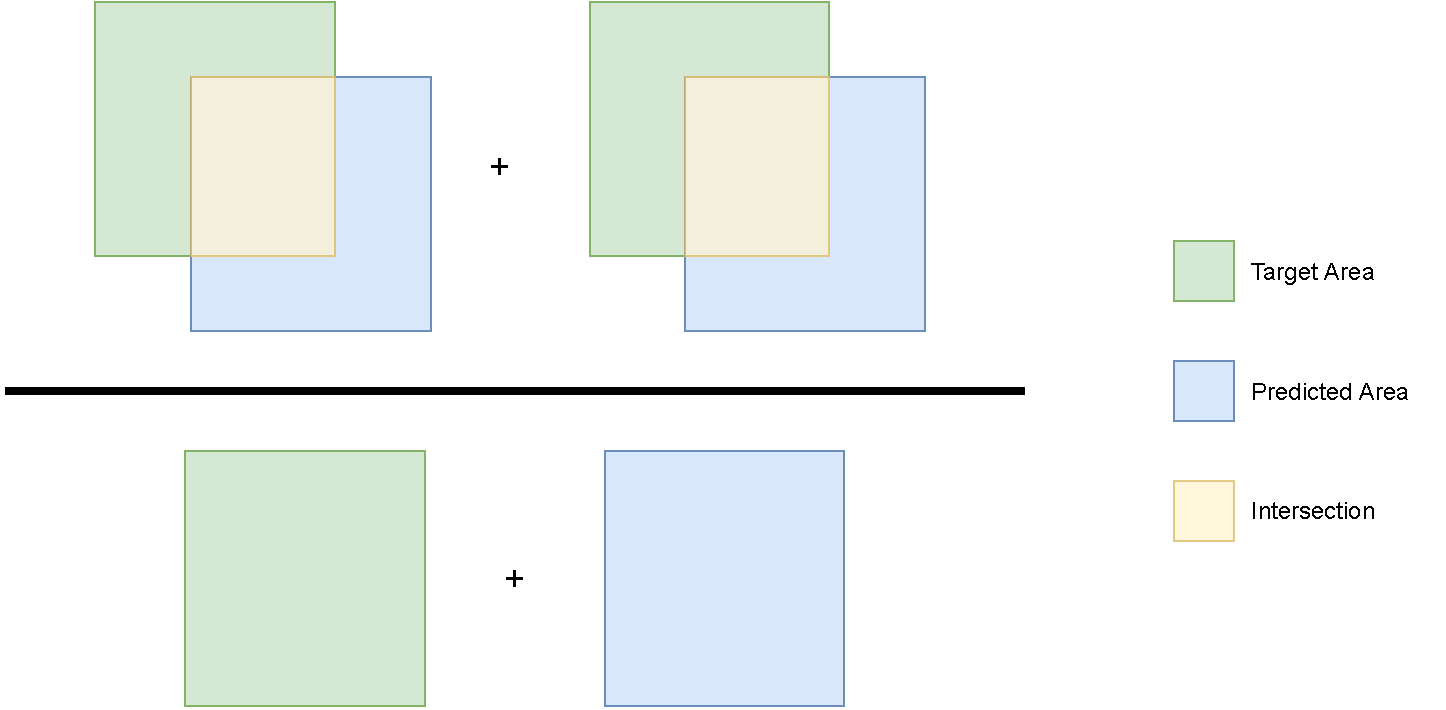
\includegraphics[width=0.9\textwidth]{img/objective_measures/dc.pdf}
  \caption{Dice Coefficient}
  \label{fig:dc}
\end{figure}